\documentclass{beamer}

\title{Data Layout and Compact Representation of BVH Trees for Raytracing}
\author{Андрей Трифонов}

\usetheme{Frankfurt}
\usepackage[main=russian,english]{babel}
\usepackage{graphicx}
\usepackage{hyperref}
\usepackage{listings}


\begin{document}

\maketitle

\begin{frame}
    \frametitle{References}
    Data Layout:
    \begin{itemize}
        \item
            \href{https://diglib.eg.org/bitstream/handle/10.2312/EGPGV.EGPGV13.057-064/057-064.pdf?sequence=1}
            {\textit{"Analysis of Cache Behavior and Performance of Different BVH Memory
            Layouts for Tracing Incoherent Rays"} by D. Wodniok, A. Schulz, S. Widmer and M. Goese}
        \item
            \href{https://sci-hub.ru/http://dx.doi.org/10.1145/2790060.2790065}
            {\textit{"Bounding Volume Hierarchy Optimization through Agglomerative Treelet Restructuring"}
            by Leonardo R. Domingues and Helio Pedrini}
    \end{itemize}
    Компактное Представление:
    \begin{itemize}
        \item
            \href{https://woizischke.com/ray-tracing-single-slab-hierarchy.pdf}
            {\textit{"Ray Tracing with the Single Slab Hierarchy"}
            by Martin Eisemann, Christian Woizischke and Marcus Magnor}
        \item
            \href{https://diglib.eg.org/bitstream/handle/10.2312/PE.VMV.VMV10.227-234/227-234.pdf}
            {\textit{"The Minimal Bounding Volume Hierarchy"}
            by Pablo Bauszat, Martin Eisemann and Marcus Magnor}
    \end{itemize}
\end{frame}

\begin{frame}
    \frametitle{Что такое BVH?}
    \begin{block}{}
        \textbf{Bounding Volume Hierarchy (BVH)} - иерархия ограничивающих объемов (BV).
    \end{block}
    \begin{figure}
        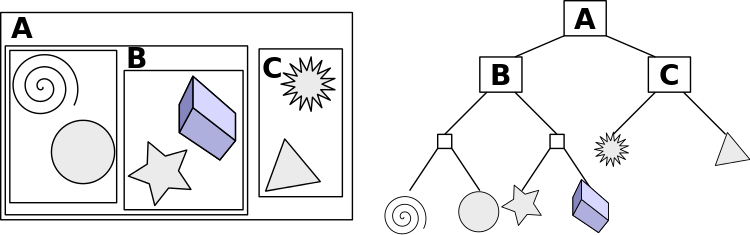
\includegraphics[keepaspectratio, width=\textwidth]{res/bvh.png}
    \end{figure}
    Все геометрические объекты, образующие листовые узлы дерева, заключены в эти BV.

    Затем эти узлы группируются в небольшие наборы и заключаются в более крупные BV.

\end{frame}

\begin{frame}
    \frametitle{Типы BV}
    \textbf{Типы ограничивающих объемов}:
    \begin{itemize}
        \item
            Sphere tree
        \item
            AABB tree (Axis Aligned Bounding Box)
        \item
            OBB tree (Oriented Bounding Box)
        \item
            k-DOP (Discrete Oriented Polytope)
        \item
            SSV (Swept Sphere Volume)
    \end{itemize}
    \begin{figure}
        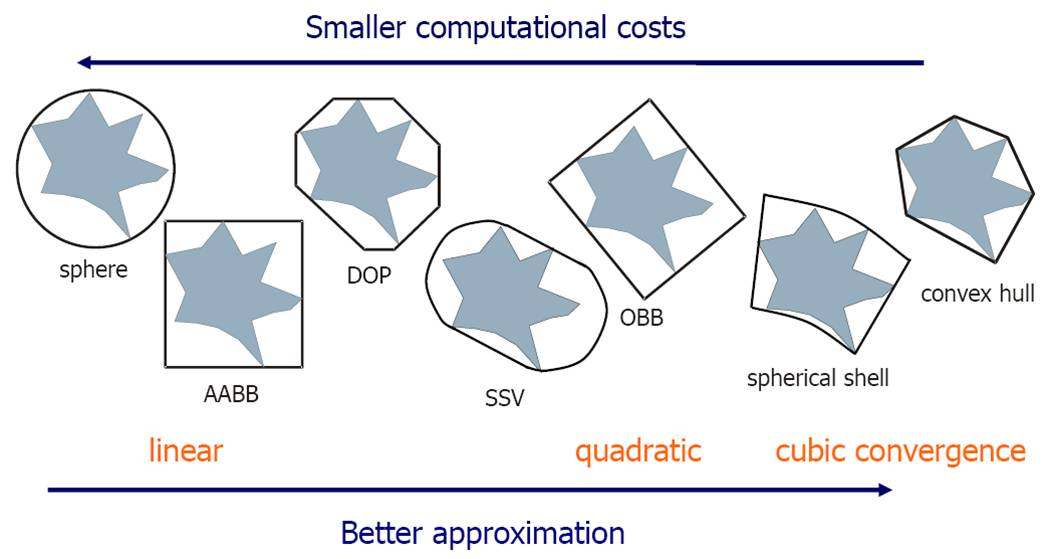
\includegraphics[keepaspectratio, width=\textwidth]{res/bvh_types.jpg}
    \end{figure}
\end{frame}

\begin{frame}
    \frametitle{BVH для трассировки лучей}
    \begin{block}{Зачем?}
        BVH часто используются в трассировке лучей для устранения потенциальных кандидатов
        на пересечение в сцене путем пропуска геометрических объектов,
        расположенных в ограничивающих объемах,
        которые не пересекаются текущим лучом.
    \end{block}
    Путем организации BV в BVH временная сложность (количество выполненных тестов)
    может быть уменьшена с линейной до логарифмической от количества примитивов (треугольников).

    В контексте ускоряющей структуры для рейтрейсинга используются:
    \begin{itemize}
        \item
            AABB (Axis Aligned Bounding Box)
        \item
            OBB (Oriented Bounding Box) \textit{(намного реже)}
    \end{itemize}


\end{frame}

\begin{frame}
    \frametitle{Метрики}
    \textbf{Для оценки эффективности BVH используются метрики}:
    \begin{itemize}
        \item
            Количество обойдённых узлов (NodesCount – NC)
        \item
            Количество обойдённых листьев (LeavesCount – LC)
        \item
            Кол-во арифметических операций проверки пересечения AABB (или др.) с лучом (AOC)
        \item
            Количество тестов луч-треугольник (или кол-во арифметических операций, TC)
        \item
            Количество длинных прыжков в пределах 1 буфера (LongJumpCount – LJC)
        \item
            Объём памяти, прочитанный (BusLoadInBytes – BLB)
        \item
            Leaf Count Variability (LCV)
        \item
            Время на определённом CPU
        \item
            Время на определённом GPU (не для всех)
        \item
            Общий объём памяти на всё дерево
    \end{itemize}
\end{frame}

\begin{frame}
    \frametitle{Функция стоимости BVH дерева}
    \begin{block}{Traversal cost \(c_T\) }
        Средняя стоимость пересечения луча c BV
    \end{block}
    \begin{block}{Intersection cost \(c_I\) }
        Средняя стоимость пересечения луча с примитивом сцены
    \end{block}
    \begin{block}{Conditional probability \(P(N_c\lvert N)\) }
        Условная вероятность пересечения дочернего узла \(N_c\) при пересеченном узле \(N\)
    \end{block}
    \begin{block}{Cost function}
        \(
        c(N) = \begin{cases}
            c_T + \displaystyle \sum_{N_c} P(N_c \lvert N)c(N_c)  \\
            c_I \lvert N \rvert\text{ \textit{(if N is leaf)} }
        \end{cases}
        \)
    \end{block}
\end{frame}

\begin{frame}
    \frametitle{Кэширование}
    \begin{block}{Cache locality CPU \& GPU}
        Когда вы обращаетесь к памяти, ее фрагменты кэшируются на разных уровнях.
        Локальность кеша относится к вероятности того,
        что последовательные операции будут находиться в кеше и,
        следовательно, будут выполняться быстрее.
    \end{block}
    \begin{block}{GPU Texture memory}
        Текстурная память GPU относится к аппаратному блоку, который мапается на глобальную память GPU.
        Этот аппаратный блок предоставляет свой механизм кэширования.
        \begin{itemize}
            \item
                максимизации 2D пространственной локальности
            \item
                аппаратная обработка адресов, выходящих за границы
        \end{itemize}
    \end{block}
\end{frame}

\begin{frame}
    \frametitle{Data layout}
    \begin{block}{Идея}
        Изменения порядка узлов и их внутреннего представления может улучшить \textbf{cache locality}
        и тем самым уменьшить \textbf{traversal cost}.
    \end{block}
\end{frame}

\begin{frame}[t]
    \frametitle{Компактное представление BVH}
    Существует несколько подходов, которые пытаются \textbf{минимизировать использование памяти}, используя один или несколько из следующих методов:
    \begin{itemize}
        \item
            Сокращение информации, которая хранится для каждого BV
        \item
            Снижение точности данных, которые хранятся в BV
        \item
            Удаление дочерних и примитивных указателей неявным индексированием
        \item
            Повышение коэффициента ветвления (числа потомков на узел), чтобы уменьшить общее количество узлов в BVH
        \item
            Сжатие данных иерархии
    \end{itemize}

\end{frame}

\begin{frame}
    \frametitle{Single Slab Hierarchy}
    \framesubtitle{Ray Tracing with the Single Slab Hierarchy}
    \textbf{The single slab hierarchy (SSH)} - это способ разделения BV надвое одной пластиной,
    в результате чего получается двоичное дерево.

    Представляем BV одной огранивающей пластиной, вместо хранения min/max для каждой из осей.

\end{frame}

\begin{frame}
    \frametitle{Enclosing Property of BVH}
    \begin{block}{}
        Ограничевающее свойство BVH обеспечивает,
        что луч всегда:
        \begin{itemize}
            \item 
                пересекает сначала (или одновременно) узел предок, прежде чем он
                сможет пересечь дочерние узлы
            \item 
                всегда будет покидать дочерние узлы
                раньше или одновременно узла-предка
        \end{itemize}
    \end{block}

    \begin{figure}
        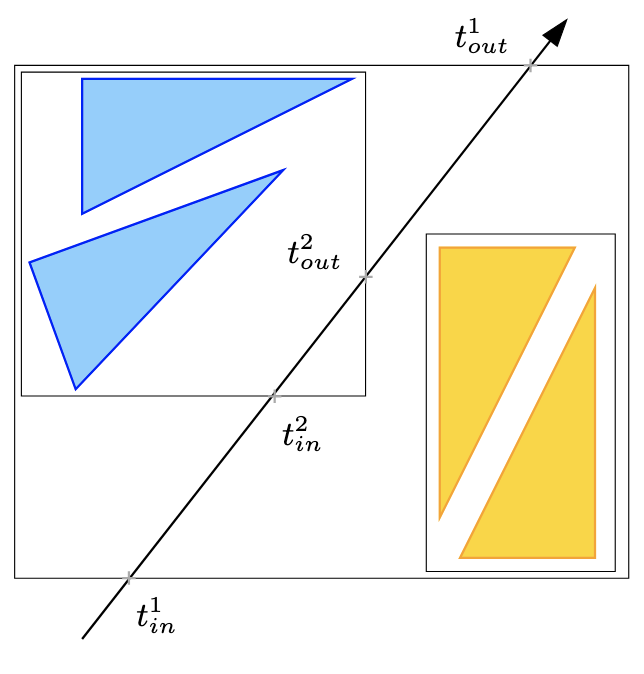
\includegraphics[keepaspectratio, height=0.5\textheight]{res/enclosing.png}
    \end{figure}

\end{frame}

\begin{frame}
    \frametitle{Bounding Plane Adjustment}
    Чтобы не оставлять пустот в BVH, для каждого дочернего узла мы подбираем
    свою ось вдоль которой разместить splitting plane (single slab).

    Значит, помимо координаты по оси нашей splitting plane, для каждого узла нужно
    хранить выбранную ось (как флаг).
    \begin{figure}
        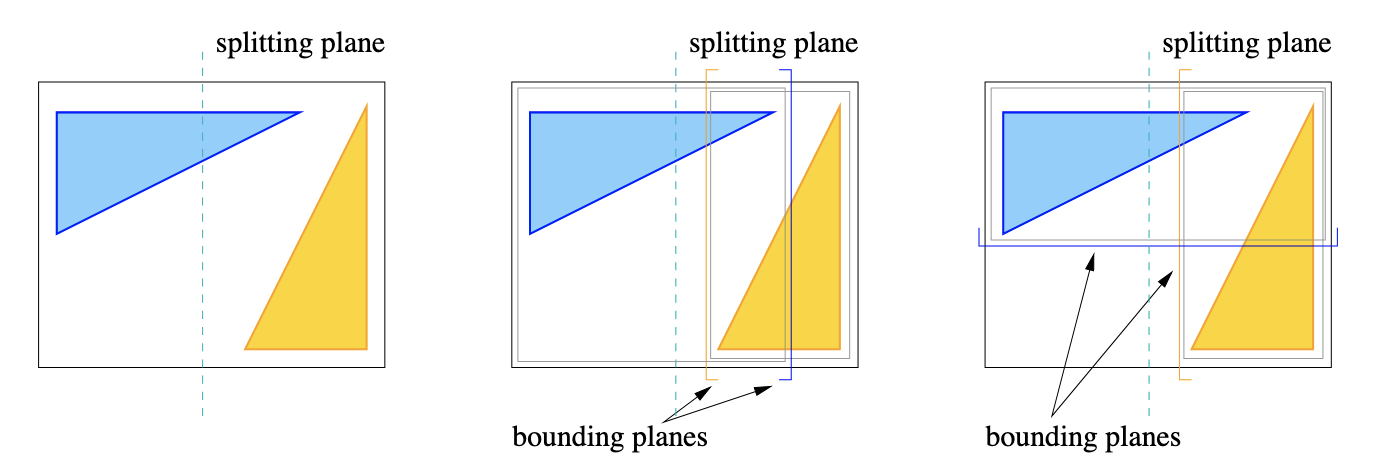
\includegraphics[keepaspectratio, width=\textwidth]{res/splitting_ssh.png}
    \end{figure}
\end{frame}

\begin{frame}
    \frametitle{Лишние вычисления}
    \begin{block}{Еще одно полезное свойство, касающееся эффективности}
        BV дочерних элементов узла имеют общие ограничивающие плоскости со своим родителем.
        По крайней мере 6/12 плоскостей, определяющие два дочерних узла, будут совпадать
        с границами родительского узла.
    \end{block}
\end{frame}

\begin{frame}[fragile]
    \frametitle{Single Slab Hierarchy}
    \framesubtitle{Структура Узла}

    \begin{semiverbatim}
        #pragma align(8)
        struct SSHNode \{
            float plane;
            union \{
                int firstChildNodeID; //inner nodes
                int firstTriangleID; //leaf nodes
                // bit 0..1: x/y/z/leaf
                // bit 2: left/right interior
                // bit 3..4: traversal axis
            \}
        \};
    \end{semiverbatim}
    Заняв 5 битов флагами у нас остается 27 битов (от int32),
    чтобы сохранить индекс.
    Таким образом можно закодировать до 134 мил. примитивов.

\end{frame}

\begin{frame}
    \frametitle{Single Slab Hierarchy}
    \framesubtitle{SAH}
    \begin{block}{SAH (surface area heuristic)}
        S(B) - surface area of node B

        \(
        P(\overrightarrow{r}\cap B^i \lvert \overrightarrow{r} \cap B^0)_{SAH} = \frac{S(B^i)}{S(B^0)}
        \)
    \end{block}

\end{frame}

\begin{frame}[fragile]
    \frametitle{Single Slab Hierarchy}
    \framesubtitle{Construction}

    \begin{lstlisting}[language=C++,basicstyle=\ttfamily,keywordstyle=\color{red}]
void createSSH(TriangleList tris, AABB parent,
                SSHNode& node) {
    AABB bounds(tris); // bounding box
    float bestSurface = HUGE_VAL;
    int bestSide = 0;
    for (Side side : make_sides(bounds)) {
        AABB temp(parent);
        temp.side = side;
        if (surface(temp) < bestSurface) {
            bestSurface = surface(temp);
            bestSide = side;
        }
    }
    ...

    \end{lstlisting}

\end{frame}

\begin{frame}[fragile]
    \frametitle{Single Slab Hierarchy}
    \framesubtitle{Construction}
    \begin{lstlisting}[language=C++,basicstyle=\ttfamily,keywordstyle=\color{red}]
    ...
    node.boundingPlane = boudns.bestSide;

    if (tris.size() < n) {
        createLeafNode(); return; }

    TriangleList leftTris, rightTris;
    subdivide(tris, leftTris, rightTris); // SAH
    parent.bestSide = boudns.bestSide;

    int childID = node.firstChildNodeID;
    createSSH(leftTris, parent, childID);
    createSSH(rightTris, parent, childID + 1);
}
    \end{lstlisting}
\end{frame}

\begin{frame}[fragile]
    \frametitle{Single Slab Hierarchy}
    \framesubtitle{Traversal}
    \begin{lstlisting}[language=C++,basicstyle=\ttfamily,keywordstyle=\color{red}]
bool intersectSSH(Ray& ray, mask reverse[3],
        SSHNode* node, float& t_hit,
        float& t_near, float& t_far) {

    // 1. Calculate the distance to its BP
    int axis = node->getSlabAxis();
    float t = (node->plane - ray.origin[axis])
        / ray.dir[axis];

    // 2. Compare it to the active ray segment
    if (node->geometryIsLeft()) {
        t_near = (reverse[axis] | (t <= t_near)) ? t_near : t;
        t_far  = (reverse[axis] & (t < t_far)) ? t : t_far;
    } else {
        t_near = (reverse[axis] & (t > t_near)) ? t_near : t;
        t_far  = (reverse[axis] | (t >= t_far)) ? t : t_far;
    }

    if ((t_near > t_far) || (t_near > t_hit)) {
        return false;
    };

    if (node->isLeaf()) {
        return intersectGeometry;
    } else {
        /*
           traverse children here
           */
    }
}
    \end{lstlisting}
\end{frame}

\begin{frame}
    \frametitle{Single Slab Hierarchy}
    \framesubtitle{Extension to dynamic scenes}
    \begin{block}{Skinned meshes}
    Можно применить простой bottom-up подход,
    используя тривиальные min/max операции для адаптации границ узлов.
    Структура иерархии остается неизменной.

    Этого достаточно для большинства когерентных анимаций.
    \end{block}

    \begin{block}{Arbitrary movements}
    Можно параллельно перестраивать SSH. Как только построение будет завершено - сделать замену.
    \end{block}

\end{frame}

\begin{frame}[t]
    \frametitle{Плюсы и минусы}
    \framesubtitle{Single Slab Hierarchy}

    \textbf{Достоинства}:
    \begin{itemize}
        \item
            Сжатие 75\%
        \item
            Подходит для интерактивного рейтрейсинга
        \item
            Возможность адаптировать под динамические сцены
        \item
            Более легкий алгоритм траверса (в 6 раз быстрее чем пересекать с AABB)
        \item
            Не изменена структура самого дерева - изменено только представление узлов
        \item
            Сравним по скорости с обычным AABB BVH
        \item
            Преобразует уже построенный AABB BVH
    \end{itemize}

    \textbf{Недостатки}:
    \begin{itemize}
        \item
            Немного дольше строить
        \item
            В два раза больше узлов проходит по сравнению с AABB BVH
        \item
            В среднем на один треугольник на луч пересекается больше
    \end{itemize}

\end{frame}

\begin{frame}[t]
    \frametitle{Результаты}
    \framesubtitle{Single Slab Hierarchy}
    \begin{columns}
        \column{0.7\textwidth}
        \begin{itemize}
            \item
                $N_T$: avg of traversed nodes per ray
            \item
                $N_I$: avg of ray-object intersections per ray
            \item
                $T_C$: total time needed for \textbf{construction}
            \item
                $T_R$: total time needed for \textbf{traversal}
            \item
                $s(T_R)$: speedup achieved by the SSH with respect to the BVH
            \item
                $Mem$: memory usage of the AS in megabytes, excluding the triangle data
        \end{itemize}
        \column{0.5\textwidth}
        \begin{figure}
            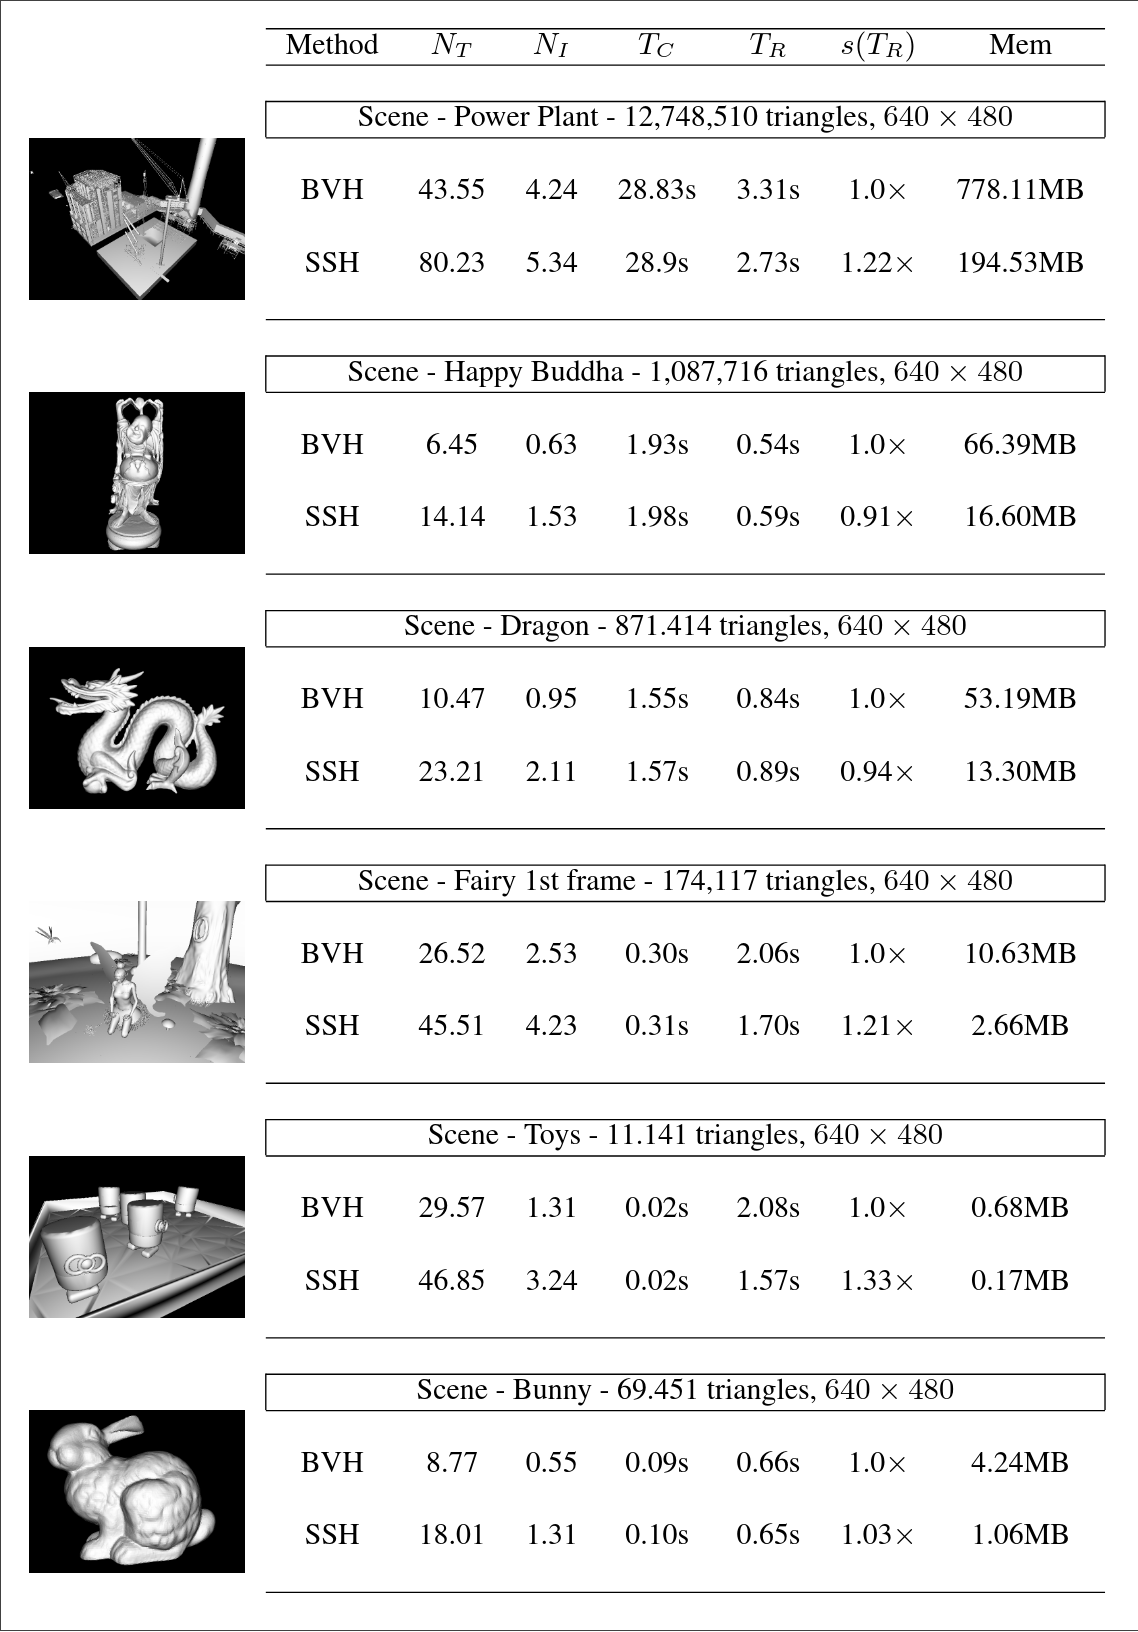
\includegraphics[keepaspectratio, height=.75\textheight]{res/results_ssh.png}
        \end{figure}
    \end{columns}

\end{frame}

\begin{frame}[t]
    \frametitle{The Minimal Bounding Volume Hierarchy}
    \begin{block}{The Minimal Bounding Volume Hierarchy (MVH)}
        Минимальная иерархия ограничевающих объемов - полное k-арное дерево BVH, которое хранится в массиве
        и индексируется как heap.
        Каждый узел либо листовой, либо имеет k дочерних.
    \end{block}
    Принципы, используемые для этого компактного представления BVH:
    \begin{itemize}
        \item
            Удаление дочерних и примитивных указателей \textbf{неявным индексированием}
        \item
            \textbf{Сокращение информации}, которая хранится для каждого BV
    \end{itemize}

\end{frame}

\begin{frame}[t]
    \frametitle{Неявное индексировние}
    \framesubtitle{Minimal Bounding Volume Hierarchy}

    \begin{columns}
        \column{0.5\textwidth}
        \begin{block}{}
            Индексы дочерних узлов $i$-ого узла между $i*k+1$ и $i*k + k$
        \end{block}

        В статье-источнике $k=2$, то есть дерево - бинарное.

        Обозначим кол-во примитивов на узел $n$. И пусть листовые узлы начинаются с индекса $l$.

        \begin{block}{}
            $primID = (i - l) * n$ - будет индекс первого примитива в массиве примитивов для $i$-го узла (если он листовой, то $i > l$).
        \end{block}
        \column{0.5\textwidth}
        \begin{figure}
            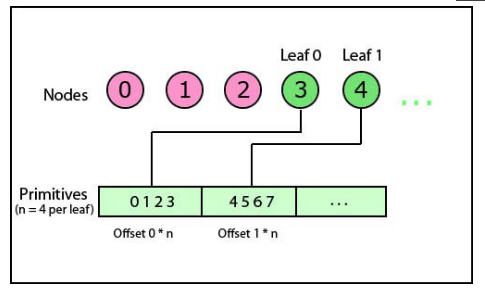
\includegraphics[keepaspectratio, width=\textwidth]{res/mem_layout_mvh.png}
        \end{figure}
        \begin{figure}
            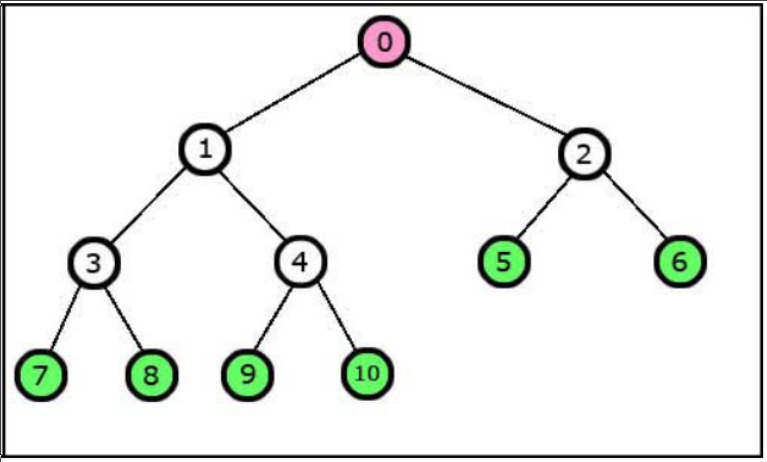
\includegraphics[keepaspectratio, width=\textwidth]{res/tree_mvh.png}
        \end{figure}
    \end{columns}

\end{frame}

\begin{frame}[t]
    \frametitle{Сокращение хранимых данных для узла MVH}
    \framesubtitle{Minimal Bounding Volume Hierarchy}
    \begin{columns}
        \column{0.7\textwidth}
        Выделим для узла всего 2 бита. Получим 4 возможных варианта для получившегося дочернего узла:
        \begin{itemize}
            \item
                No-Cut: if no surface reduction is possible for this node
            \item
                Left-Cut: if the minimum slab is increased
            \item
                Right-Cut: if the maximum slab is decreased
            \item
                Both-Cut: if the Left-Cut and Right-Cut is used
        \end{itemize}
        \column{0.3\textwidth}
        \begin{figure}
            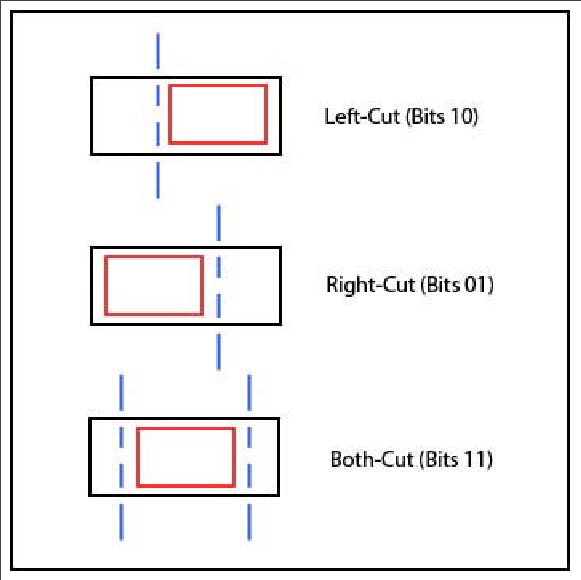
\includegraphics[keepaspectratio, width=\textwidth]{res/splitting_mvh.png}
        \end{figure}
    \end{columns}

    \begin{block}{}
        Каждый раз мы используем фиксированный reduction factor $\zeta$
        Лучшие результаты с $\zeta \in [ 0.35, 0.30]$
    \end{block}

\end{frame}

\begin{frame}
    \frametitle{Построение MVH. Алгоритм}
    \framesubtitle{Minimal Bounding Volume Hierarchy}
    \begin{enumerate}
        \item
            Дублируем последний примитив пока $P$ не станет $ P \% n = 0$
        \item
            Сколько узлов всего? Для $k = 2$ кол-во узлов $2(P/n) -1$
        \item
            Сколько узлов в каждом поддереве?
            \begin{itemize}
                \item[$-$]
                    Присваиваем всем листьям их кол-во примитивов
                \item[$-$]
                    Суммируем bottom-up, пока не дойдем до корня
            \end{itemize}
        \item
            Пусть всего $N$ узлов. Тогда аллоцируем массив длины $2N$ из \textit{int32}
        \item
            MVH строится с использованием object median split, где
            процесс разделения использует предварительно вычисленные количества примитивов для
            разделения списка объектов на две части
    \end{enumerate}
    
\end{frame}

\begin{frame}
    \frametitle{Построение MVH. Алгоритм (продолжение)}
    \framesubtitle{Minimal Bounding Volume Hierarchy}
    \begin{enumerate}
        \item 
            aa
    \end{enumerate}
\end{frame}

\end{document}
